% Provenance (never printed): old premiere S material on magmatic rocks (volcanic
% and plutonic textures and cooling rate; basalt/gabbro, andesite/diorite,
% rhyolite/granite; order of crystallisation, told). Cooling of sheets from
% figdata/grade-11/dyke_cooling.py (Delaney 1986 parameters; kappa from England
% et al. 2007). Fractional crystallisation is Year 2's; metamorphism (contact
% aureoles) is g12.03's: not developed here.
\chapter{आग्नेय चट्टानें}\label{ch:g11:igneous-rocks}

आयरलैंड के उत्तरी तट पर, अगल-बगल सटे पत्थर के स्तंभ सीढ़ियों की तरह समुद्र में
उतरते हैं: जायंट्स कॉज़वे, एक बेसाल्ट जो
किसी लावा से ठंडा होकर बना। कैलिफ़ोर्निया के योसेमिटी में एल
कैपिटन की ग्रेनाइट दीवार घाटी की तली से लगभग \qty{900}{m} ऊपर उठती है, मोटे कणों वाली
चट्टान का एक अकेला पिंड। दोनों मैग्मा से क्रिस्टलित हुए। बेसाल्ट
सतह पर ठंडा हुआ, उसके क्रिस्टल देखने के लिए बहुत छोटे हैं; ग्रेनाइट भूमि के बहुत नीचे ठंडा हुआ,
उसके क्रिस्टल देखने लायक बड़े हैं, और वह आज केवल इसलिए दिखता है कि
उसके ऊपर की चट्टानें घिसकर हट गई हैं। यह अध्याय किसी चट्टान के कणों में
पढ़ता है कि वह कितनी तेज़ी से, और कितनी गहराई पर, ठंडी हुई।
% ledger: photo:g11-giants-causeway, photo:g11-el-capitan, tulane:intrusions

\begin{omfigure}
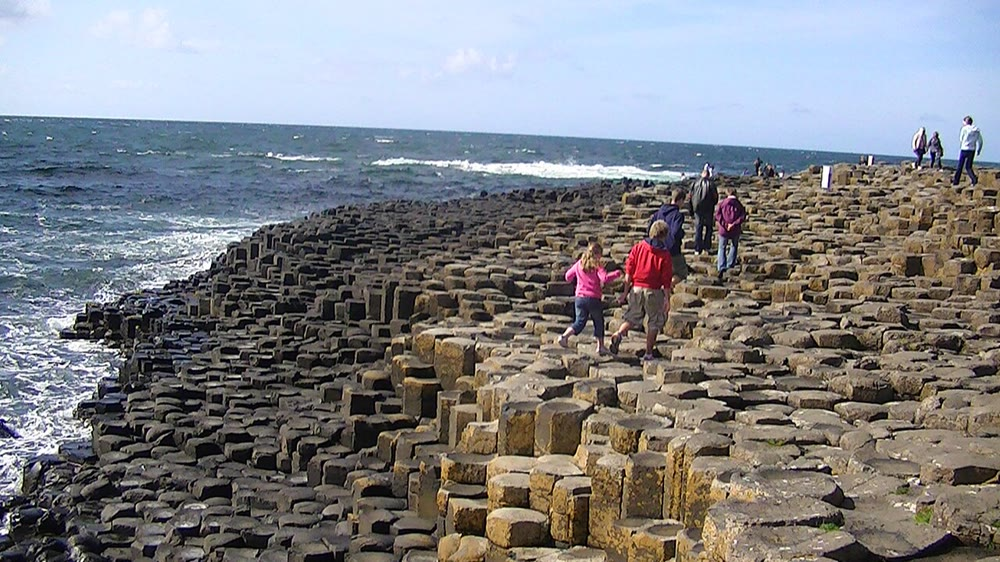
\includegraphics[height=4.3cm]{images/book2/g11-bishop-giants-causeway.jpg}\hspace{0.04\linewidth}%
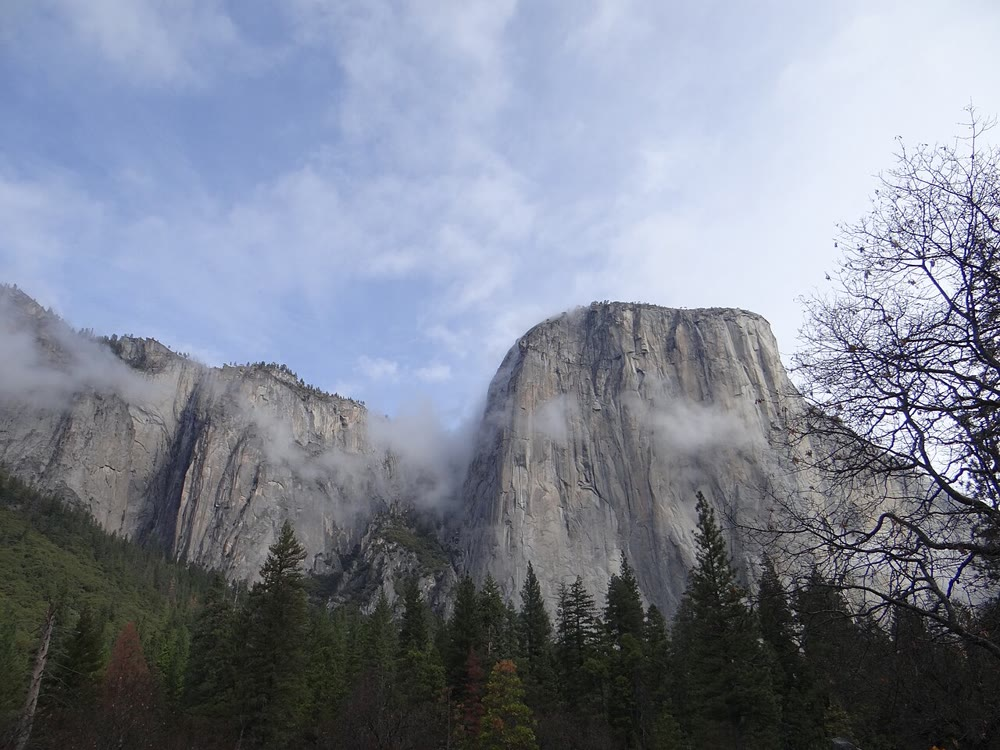
\includegraphics[height=4.3cm]{images/book2/g11-usgs-el-capitan.jpg}

{\small बाएँ: उत्तरी आयरलैंड के जायंट्स कॉज़वे के बेसाल्ट स्तंभ।
फ़ोटो ऐडम बिशप (CC~BY-SA~3.0)। दाएँ: योसेमिटी, कैलिफ़ोर्निया का एल कैपिटन,
लगभग \qty{900}{m} ऊँची ग्रेनाइट की एक दीवार। फ़ोटो अमेरिकी
भूवैज्ञानिक सर्वेक्षण (CC0)।}
\end{omfigure}
% ledger: photo:g11-giants-causeway, photo:g11-el-capitan

\begin{recall}
मैग्मा सतह के नीचे पिघली चट्टान है; वह लावा के रूप में फूटता है, शांत ढंग से या
विस्फोट के साथ (पुस्तक 1, कक्षा 7)। आग्नेय चट्टान वह है जो पिघली
चट्टान के ठंडा होकर ठोस बनने पर बनती है (पुस्तक 1, कक्षा 6)। बेसाल्ट गहरे रंग की \omterm{def:g11:igneous-rocks:volcanic-plutonic}{ज्वालामुखीय चट्टान} है, ग्रेनाइट
फ़ेल्डस्पार, क्वार्ट्ज़ और अभ्रक से बनी हल्के रंग की चट्टान (पुस्तक 1, कक्षा 6)। प्रावार का
\omterm{def:g11:ocean-ridges:peridotite}{पेरिडोटाइट} किसी कटक के नीचे ऊपर उठते हुए आंशिक रूप से पिघलता है, और \omterm{def:g11:ocean-ridges:oceanic-lithosphere}{महासागरीय भूपर्पटी} का बेसाल्ट और
\omterm{def:g11:ocean-ridges:gabbro}{गैब्रो} देता है (\cref{ch:g11:ocean-ridges})। \omterm{def:g11:minerals:rock-forming}{शैलकारी
सिलिकेट} ओलिवीन, पाइरॉक्सीन, ऐम्फ़िबोल, अभ्रक, फ़ेल्डस्पार और क्वार्ट्ज़ हैं;
फ़ेल्डस्पार हैं पोटैशियम फ़ेल्डस्पार और प्लेजियोक्लेज़, जो कैल्सियम-समृद्ध से
सोडियम-समृद्ध तक की एक श्रेणी है (\cref{ch:g11:minerals})। ऊष्मा चालन द्वारा
लगभग $\sqrt{\kappa t}$ की दूरी तक फैलती है, समय $t$ में, जहाँ
$\kappa$ ऊष्मीय विसरणशीलता है (\cref{ch:g11:subduction-zones})।
\end{recall}
% ledger: tulane:ridge-rocks, england:kelvin

\section{ज्वालामुखीय और पातालीय चट्टानें}

\begin{definition}[ज्वालामुखीय चट्टान; पातालीय चट्टान]\label{def:g11:igneous-rocks:volcanic-plutonic}
मैग्मा के क्रिस्टलन से बनी आग्नेय चट्टान
\emph{ज्वालामुखीय}\index{ज्वालामुखीय चट्टान}
(या बहिर्वेधी) होती है जब मैग्मा पृथ्वी की सतह पर, लावा के रूप में, ठोस हुआ,
और \emph{पातालीय}\index{पातालीय चट्टान} (या अंतर्वेधी) जब वह
गहराई पर, दूसरी चट्टानों के भीतर, क्रिस्टलित हुआ।
\end{definition}
% ledger: tulane:magma-types

अंतर क्रिस्टलों के आकार में दिखता है। क्रिस्टल अपने चारों ओर के द्रव से लिए गए
परमाणु जोड़कर बढ़ता है, और इसमें समय लगता है। सतह पर
लावा अपनी ऊष्मा हवा या पानी को तेज़ी से खोता है: हवा या पानी में फूटा पदार्थ
सेकंडों में ठंडा होता है, लावा-प्रवाह दिनों से हफ़्तों में। गहराई में
आसपास की चट्टानें गरम होती हैं और मैग्मा अपनी ऊष्मा धीरे-धीरे खोता है: कोई उथला
\omterm{def:g11:igneous-rocks:intrusion}{अंतर्वेधन} महीनों से वर्षों में ठंडा होता है, कोई बड़ा गहरा \omterm{def:g11:igneous-rocks:intrusion}{अंतर्वेधन} कई मिलियन
वर्ष ले सकता है। तेज़ शीतलन बहुत-से छोटे क्रिस्टल देता है, या कोई भी नहीं; धीमा शीतलन
कम, कहीं बड़े क्रिस्टल देता है।
% ledger: tulane:cooling-times, tulane:textures

\begin{definition}[गठन]\label{def:g11:igneous-rocks:texture}
किसी चट्टान का \emph{गठन}\index{गठन (चट्टान का)} उसके कणों का आकार, आकृति
और व्यवस्था है। आग्नेय चट्टान \emph{काचीय} होती है जब
उसमें कोई क्रिस्टल नहीं होते, \emph{सूक्ष्मकणी} जब उसके क्रिस्टल नंगी आँख से अलग
पहचाने जाने के लिए बहुत छोटे हों, और \emph{स्थूलकणी} जब वे सब
देखे जा सकें।
\end{definition}
% ledger: tulane:textures

कोई क्रिस्टल बढ़ पाने से पहले ही बुझा दिया गया लावा काँच बन जाता है: ऑब्सीडियन, काला
और काँच जैसा, बोतल के शंखाभ \omterm{def:g11:minerals:cleavage}{विभंग} के साथ टूटता है। बेसाल्ट
सूक्ष्मकणी है: हाथ में उसके खनिज पहचाने नहीं जा सकते, और \omterm{def:g11:minerals:thin-section}{पतली
काट} में भी क्रिस्टल छोटे होते हैं (\cref{ch:g11:minerals} का बेसाल्ट)।
ग्रेनाइट, \omterm{def:g11:ocean-ridges:gabbro}{गैब्रो} और \omterm{def:g11:igneous-rocks:rock-names}{डायोराइट} स्थूलकणी हैं: हर कण दिखता है।
% ledger: photo:g11-obsidian, photo:g11-basalt, tulane:textures

\begin{definition}[दीर्घक्रिस्टल; पोर्फ़िरी]\label{def:g11:igneous-rocks:porphyritic}
\emph{दीर्घक्रिस्टल}\index{दीर्घक्रिस्टल} कहीं छोटे क्रिस्टलों या काँच के एक पुंज,
\emph{आधार-द्रव्य}, में जड़ा एक बड़ा क्रिस्टल है। दीर्घक्रिस्टलों वाली
चट्टान \emph{पोर्फ़िरी}\index{पोर्फ़िरी} होती है।
\end{definition}
% ledger: tulane:textures

\omterm{def:g11:igneous-rocks:porphyritic}{पोर्फ़िरी} \omterm{def:g11:igneous-rocks:texture}{गठन} शीतलन की दो अवस्थाएँ दर्ज करता है: पहले धीमी, गहराई पर,
जब \omterm{def:g11:igneous-rocks:porphyritic}{दीर्घक्रिस्टल} ऐसे मैग्मा में बढ़े जो अब भी ज़्यादातर द्रव था; फिर
तेज़, जब मैग्मा ऊपर उठकर फूटा, या ठंडी चट्टान में अंतःक्षिप्त हुआ, और
शेष द्रव जमकर आधार-द्रव्य बन गया।
% ledger: tulane:textures

\begin{omfigure}
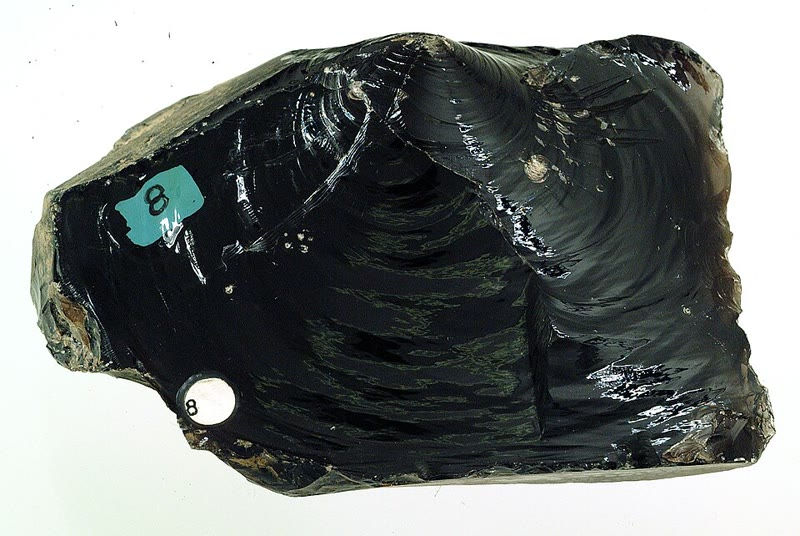
\includegraphics[height=2.75cm]{images/book2/g11-geodil-obsidian.jpg}\hfill
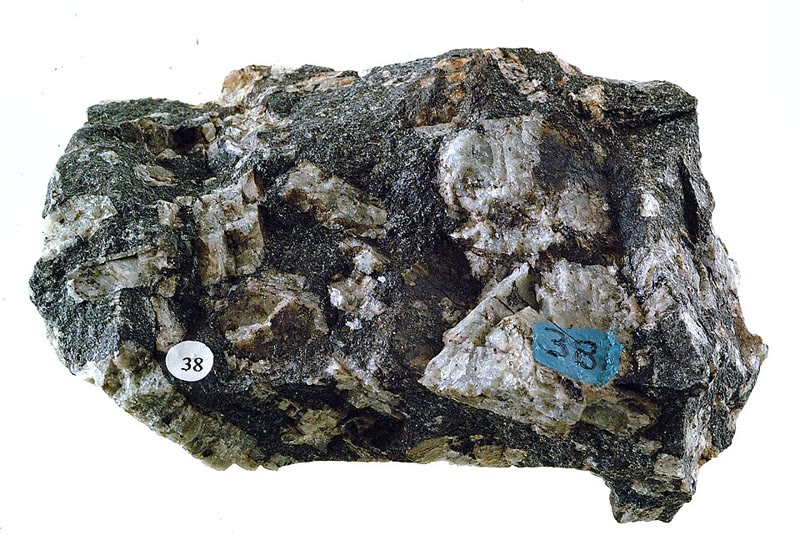
\includegraphics[height=2.75cm]{images/book2/g11-geodil-diabase-porphyry.jpg}\hfill
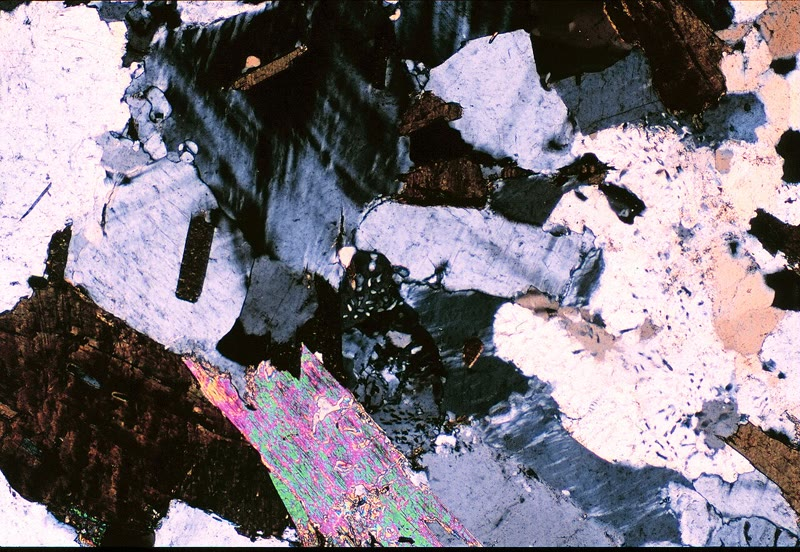
\includegraphics[height=2.75cm]{images/book2/g11-geodil-granite-xpl.jpg}\hfill
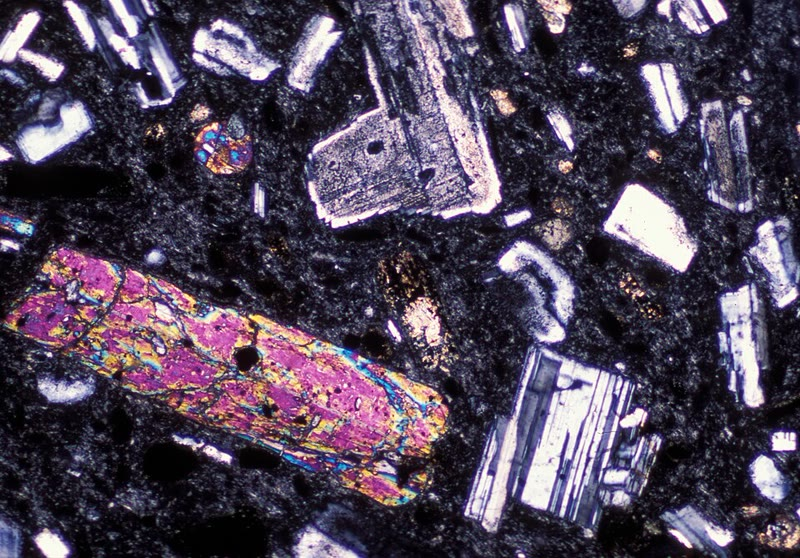
\includegraphics[height=2.75cm]{images/book2/g11-geodil-andesite-xpl.jpg}

{\small बाएँ से दाएँ: ऑब्सीडियन, एक \omterm{def:g11:igneous-rocks:volcanic-plutonic}{ज्वालामुखीय} काँच, अपने वक्र
शंखाभ \omterm{def:g11:minerals:cleavage}{विभंग} के साथ (\qty{9.5}{cm} चौड़ा); एक \omterm{def:g11:igneous-rocks:porphyritic}{पोर्फ़िरी} चट्टान, अधिक बारीक आधार-द्रव्य में
प्लेजियोक्लेज़ के खंड जैसे \omterm{def:g11:igneous-rocks:porphyritic}{दीर्घक्रिस्टल} (\qty{9}{cm}); फिर व्यत्यस्त ध्रुवकों के बीच दो
\omterm{def:g11:minerals:thin-section}{पतली काटें}: एक ग्रेनाइट, सभी कण बड़े और
आपस में गुँथे --- भूरा बायोटाइट, चटकीले रंग का एक मस्कोवाइट, धारीदार
प्लेजियोक्लेज़, धूसर और सफ़ेद क्वार्ट्ज़; एक \omterm{def:g11:igneous-rocks:rock-names}{एंडेसाइट}, सूक्ष्मकणी आधार-द्रव्य में
प्लेजियोक्लेज़ और ऐम्फ़िबोल के \omterm{def:g11:igneous-rocks:porphyritic}{दीर्घक्रिस्टल}। फ़ोटो ट्वायला
बेकर, माइक डेविस और डार्ला सॉन्ड्रोल, भूविज्ञान डिजिटल छवि पुस्तकालय (CC0)।}
\end{omfigure}
% ledger: photo:g11-obsidian, photo:g11-diabase-porphyry, photo:g11-granite-xpl, photo:g11-andesite-xpl

\section{आग्नेय चट्टानों का नामकरण}

आग्नेय चट्टान की दूसरी कुंजी उसका रसायन है, और सबसे बढ़कर उसमें
सिलिका, \ce{SiO2}, की मात्रा, जो सामान्य मैग्माओं में द्रव्यमान के लगभग
\qty{45}{\percent} से लगभग \qty{75}{\percent} तक होती है।

\begin{definition}[मैफ़िक; मध्यवर्ती; फ़ेल्सिक]\label{def:g11:igneous-rocks:felsic-mafic}
कोई मैग्मा, या उससे बनी चट्टान, \emph{मैफ़िक}\index{मैफ़िक} होती है जब उसमें
लगभग \qty{45}{\percent} से \qty{55}{\percent} \ce{SiO2} हो और वह
लोहे, मैग्नीशियम और कैल्सियम से समृद्ध हो; \emph{मध्यवर्ती}\index{मध्यवर्ती (चट्टान)}
जब \qty{55}{\percent} और \qty{65}{\percent} के बीच; \emph{फ़ेल्सिक}\index{फ़ेल्सिक}
जब उसमें लगभग \qty{65}{\percent} से \qty{75}{\percent} \ce{SiO2} हो और वह
लोहे, मैग्नीशियम और कैल्सियम में निर्धन पर सोडियम और पोटैशियम से समृद्ध हो।
\end{definition}
% ledger: tulane:magma-types, earle:magma-oxides

हर प्रकार का मैग्मा दो चट्टानें देता है, एक \omterm{def:g11:igneous-rocks:volcanic-plutonic}{ज्वालामुखीय} और सूक्ष्मकणी, एक
\omterm{def:g11:igneous-rocks:volcanic-plutonic}{पातालीय} और स्थूलकणी, एक ही रसायन वाली। बेसाल्ट और \omterm{def:g11:ocean-ridges:gabbro}{गैब्रो}
\omterm{def:g11:igneous-rocks:felsic-mafic}{मैफ़िक} जोड़ी हैं, जो \omterm{def:g11:ocean-ridges:oceanic-lithosphere}{महासागरीय भूपर्पटी} के साथ मिलीं; ग्रेनाइट \omterm{def:g11:igneous-rocks:felsic-mafic}{फ़ेल्सिक} \omterm{def:g11:igneous-rocks:volcanic-plutonic}{पातालीय
चट्टान} है। तीन नाम समुच्चय पूरा करते हैं।

\begin{definition}[एंडेसाइट; डायोराइट; रायोलाइट]\label{def:g11:igneous-rocks:rock-names}
\emph{एंडेसाइट}\index{एंडेसाइट} और \emph{डायोराइट}\index{डायोराइट}
\omterm{def:g11:igneous-rocks:felsic-mafic}{मध्यवर्ती} संघटन की \omterm{def:g11:igneous-rocks:volcanic-plutonic}{ज्वालामुखीय} और \omterm{def:g11:igneous-rocks:volcanic-plutonic}{पातालीय चट्टानें} हैं, जो ज़्यादातर
प्लेजियोक्लेज़ और ऐम्फ़िबोल या पाइरॉक्सीन से बनी हैं। \emph{रायोलाइट}\index{रायोलाइट}
\omterm{def:g11:igneous-rocks:felsic-mafic}{फ़ेल्सिक} संघटन की \omterm{def:g11:igneous-rocks:volcanic-plutonic}{ज्वालामुखीय चट्टान} है, ग्रेनाइट का
सूक्ष्मकणी समतुल्य।
\end{definition}
% ledger: tulane:magma-types, earle:bowen, photo:g11-andesite, photo:g11-diorite

\begin{omfigure}
\begin{tikzpicture}[font=\footnotesize, x=0.4cm]
  % columns: SiO2 45 to 75 % mapped to x = 45 to 75 (0.4 cm per %)
  \begin{scope}[xshift=-18cm]
  \fill[omLithBasalt!45] (45,0) rectangle (55,2.4);
  \fill[omLithBasalt!20] (55,0) rectangle (65,2.4);
  \fill[omLithGranite!45] (65,0) rectangle (75,2.4);
  \draw[black!60] (45,0) rectangle (75,2.4);
  \draw[black!60] (55,0) -- (55,2.4); \draw[black!60] (65,0) -- (65,2.4);
  \draw[black!60] (45,1.2) -- (75,1.2);
  \foreach \x/\a/\b in {50/बेसाल्ट/गैब्रो, 60/एंडेसाइट/डायोराइट, 70/रायोलाइट/ग्रेनाइट}{
    \node[font=\small\bfseries, text height=1.6ex, text depth=0.3ex] at (\x,1.8) {\a};
    \node[font=\small\bfseries, text height=1.6ex, text depth=0.3ex] at (\x,0.6) {\b};}
  \node[anchor=east, align=right] at (44.4,1.8) {सूक्ष्मकणी\\(ज्वालामुखीय)};
  \node[anchor=east, align=right] at (44.4,0.6) {स्थूलकणी\\(पातालीय)};
  \node[anchor=south] at (50,2.45) {मैफ़िक};
  \node[anchor=south] at (60,2.45) {मध्यवर्ती};
  \node[anchor=south] at (70,2.45) {फ़ेल्सिक};
  % minerals (a drawing: where each mineral is common)
  \foreach \y/\a/\b/\m/\c in {-0.55/45.2/52/ओलिवीन/omLithBasalt!80!black,
      -1.15/45.2/61/पाइरॉक्सीन/omLithBasalt!65!black,
      -1.75/52/69/ऐम्फ़िबोल/black!60,
      -2.35/57/74.8/बायोटाइट/black!75,
      -2.95/45.2/72/प्लेजियोक्लेज़/omDef!45,
      -3.55/63/74.8/पोटैशियम फ़ेल्डस्पार/omLithGranite!90!red,
      -4.15/64/74.8/क्वार्ट्ज़/black!20,
      -4.75/68/74.8/मस्कोवाइट/black!35}{
    \fill[\c] (\a,\y) .. controls ({\a+1.2},{\y+0.22}) and ({\b-1.2},{\y+0.22}) .. (\b,\y)
              .. controls ({\b-1.2},{\y-0.22}) and ({\a+1.2},{\y-0.22}) .. (\a,\y) -- cycle;
    \node[anchor=east] at (44.4,\y) {\m};}
  \node[font=\scriptsize, text=black!75] at (50,-2.95) {कैल्सियम-समृद्ध};
  \node[font=\scriptsize, text=omDef!80!black, anchor=west] at (72.3,-2.95) {सोडियम-समृद्ध};
  % SiO2 axis
  \draw[-{Stealth[length=4pt]}] (45,-5.35) -- (75.8,-5.35);
  \foreach \x in {45,50,...,75} {\draw (\x,-5.35) -- (\x,-5.45); \node[anchor=north] at (\x,-5.45) {\x};}
  \node[anchor=north] at (60,-5.85) {\ce{SiO2} (द्रव्यमान का \unit{\percent})};
  \draw[black!30, dashed] (55,0) -- (55,-5.35); \draw[black!30, dashed] (65,0) -- (65,-5.35);
  \end{scope}
\end{tikzpicture}

{\small सामान्य आग्नेय चट्टानों का नामकरण (चित्र)। स्तंभ: मैग्मा में सिलिका
की मात्रा; पंक्तियाँ: सूक्ष्मकणी (\omterm{def:g11:igneous-rocks:volcanic-plutonic}{ज्वालामुखीय}) और स्थूलकणी
(\omterm{def:g11:igneous-rocks:volcanic-plutonic}{पातालीय}) चट्टानें। नीचे, जहाँ हर शैलकारी खनिज सामान्य है: ओलिवीन
और पाइरॉक्सीन \omterm{def:g11:igneous-rocks:felsic-mafic}{मैफ़िक} चट्टानों में कैल्सियम-समृद्ध प्लेजियोक्लेज़ के साथ; ऐम्फ़िबोल और
प्लेजियोक्लेज़ \omterm{def:g11:igneous-rocks:felsic-mafic}{मध्यवर्ती} चट्टानों में; पोटैशियम फ़ेल्डस्पार, क्वार्ट्ज़,
सोडियम-समृद्ध प्लेजियोक्लेज़ और अभ्रक \omterm{def:g11:igneous-rocks:felsic-mafic}{फ़ेल्सिक} चट्टानों में। सीमाएँ
क्रमिक हैं।}
\end{omfigure}
% ledger: tulane:magma-types, earle:bowen, earle:magma-oxides, photo:g11-andesite, photo:g11-diorite, photo:g11-granite, nps:granite-minerals

\begin{method}[आग्नेय चट्टान का नामकरण]\label{met:g11:igneous-rocks:naming}
\begin{enumerate}
  \item \omterm{def:g11:igneous-rocks:texture}{गठन} देखिए: काचीय, सूक्ष्मकणी या स्थूलकणी;
        \omterm{def:g11:igneous-rocks:porphyritic}{पोर्फ़िरी} है या नहीं। सूक्ष्मकणी या काचीय का अर्थ है \omterm{def:g11:igneous-rocks:volcanic-plutonic}{ज्वालामुखीय} (या कोई
        छोटा, जल्दी ठंडा हुआ \omterm{def:g11:igneous-rocks:intrusion}{अंतर्वेधन}); स्थूलकणी का अर्थ है \omterm{def:g11:igneous-rocks:volcanic-plutonic}{पातालीय}।
  \item जो खनिज दिख सकते हैं, उन्हें पहचानिए
        (\cref{met:g11:minerals:identify}): क्वार्ट्ज़ और पोटैशियम फ़ेल्डस्पार
        \omterm{def:g11:igneous-rocks:felsic-mafic}{फ़ेल्सिक} की ओर संकेत करते हैं, प्लेजियोक्लेज़ के साथ ऐम्फ़िबोल \omterm{def:g11:igneous-rocks:felsic-mafic}{मध्यवर्ती} की ओर, ओलिवीन
        और पाइरॉक्सीन \omterm{def:g11:igneous-rocks:felsic-mafic}{मैफ़िक} की ओर। सूक्ष्मकणी चट्टान में \omterm{def:g11:igneous-rocks:porphyritic}{दीर्घक्रिस्टलों} का,
        आधार-द्रव्य के रंग का --- \omterm{def:g11:igneous-rocks:felsic-mafic}{मैफ़िक} के लिए गहरा, \omterm{def:g11:igneous-rocks:felsic-mafic}{फ़ेल्सिक} के लिए हल्का ---
        संकेत के रूप में, या किसी रासायनिक विश्लेषण का उपयोग कीजिए।
  \item आरेख की पंक्ति और स्तंभ के मिलन-बिंदु पर नाम
        पढ़िए।
\end{enumerate}
\end{method}

\begin{example}[दो बेसाल्ट]
किसी लावा-प्रवाह की एक गहरे रंग की चट्टान पूरी तरह सूक्ष्मकणी है; उसी
ज्वालामुखी की एक दूसरी चट्टान गहरे आधार-द्रव्य में कुछ मिलीमीटर चौड़े ओलिवीन के हरे कण
दिखाती है। दोनों \omterm{def:g11:igneous-rocks:felsic-mafic}{मैफ़िक} और सूक्ष्मकणी हैं: दोनों बेसाल्ट हैं।
दूसरी \omterm{def:g11:igneous-rocks:porphyritic}{पोर्फ़िरी} बेसाल्ट है: उसका ओलिवीन पहले, धीरे-धीरे, ज्वालामुखी के नीचे के
मैग्मा में बढ़ा, इससे पहले कि लावा फूटा और उसके चारों ओर जम गया।
\end{example}
% ledger: photo:g11-olivine, earle:bowen, tulane:textures

\begin{omfigure}
\makebox[0.32\linewidth]{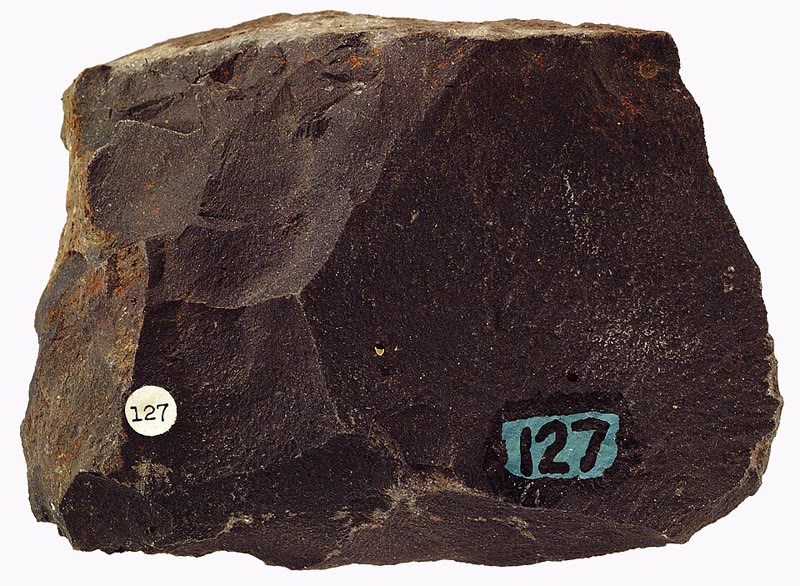
\includegraphics[height=2.9cm]{images/book2/g11-geodil-basalt.jpg}}\hfill
\makebox[0.32\linewidth]{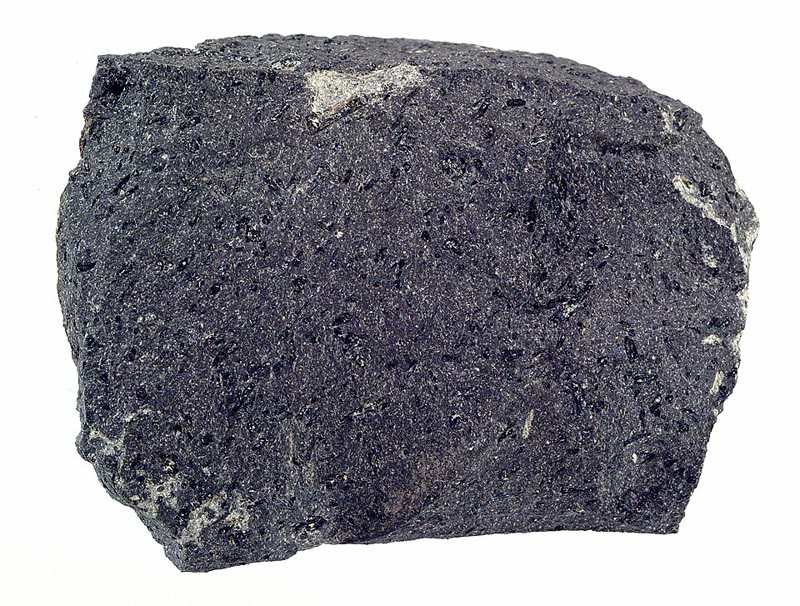
\includegraphics[height=2.9cm]{images/book2/g11-geodil-andesite.jpg}}\hfill
\makebox[0.32\linewidth]{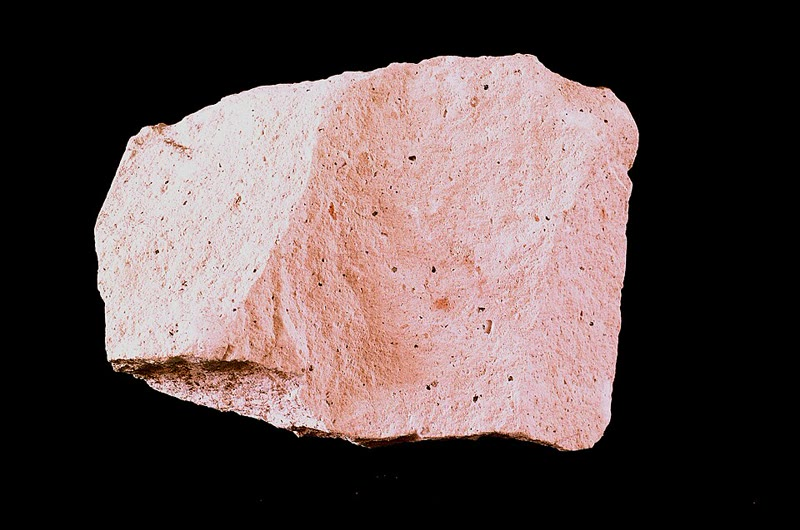
\includegraphics[height=2.9cm]{images/book2/g11-geodil-rhyolite.jpg}}

\smallskip
\makebox[0.32\linewidth]{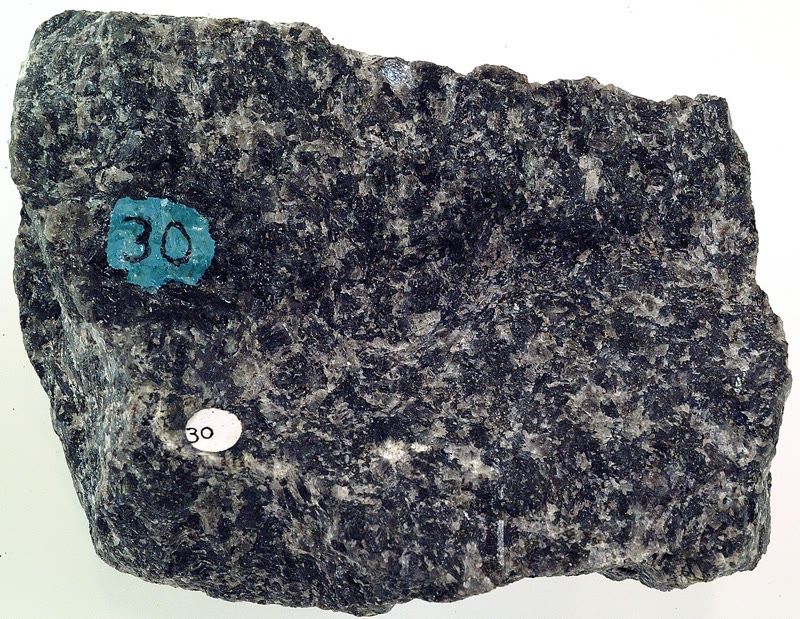
\includegraphics[height=2.9cm]{images/book2/g11-geodil-gabbro.jpg}}\hfill
\makebox[0.32\linewidth]{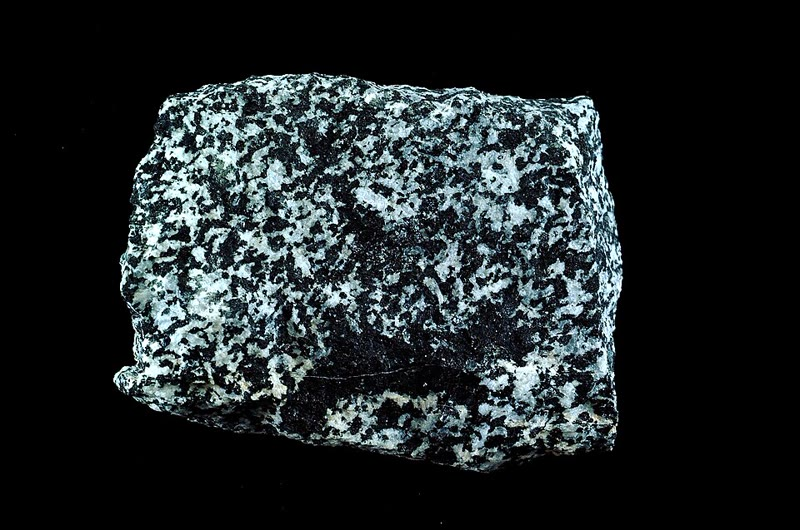
\includegraphics[height=2.9cm]{images/book2/g11-geodil-diorite.jpg}}\hfill
\makebox[0.32\linewidth]{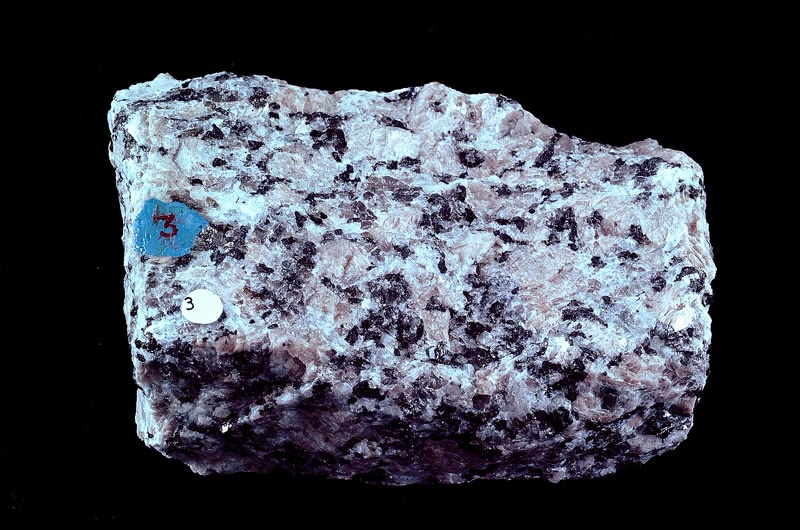
\includegraphics[height=2.9cm]{images/book2/g11-geodil-granite.jpg}}

{\small आग्नेय चट्टानों की तीन जोड़ियाँ, बाएँ से दाएँ \omterm{def:g11:igneous-rocks:felsic-mafic}{मैफ़िक} से \omterm{def:g11:igneous-rocks:felsic-mafic}{फ़ेल्सिक} तक:
ऊपर \omterm{def:g11:igneous-rocks:volcanic-plutonic}{ज्वालामुखीय}, नीचे \omterm{def:g11:igneous-rocks:volcanic-plutonic}{पातालीय}। ऊपर: एक सूक्ष्मकणी बेसाल्ट; एक \omterm{def:g11:igneous-rocks:rock-names}{एंडेसाइट}, सूक्ष्मकणी
आधार-द्रव्य में ऐम्फ़िबोल के छोटे क्रिस्टल (लगभग \qty{10}{cm});
एक गुलाबी \omterm{def:g11:igneous-rocks:rock-names}{रायोलाइट}। नीचे: \omterm{def:g11:ocean-ridges:gabbro}{गैब्रो} (\qty{9}{cm}); \omterm{def:g11:igneous-rocks:rock-names}{डायोराइट}, काला हॉर्नब्लेंड और
काँच जैसा प्लेजियोक्लेज़ (\qty{10}{cm}); एक मोटे कणों वाला ग्रेनाइट, हल्के गुलाबी बड़े
पोटैशियम फ़ेल्डस्पारों, धूसर प्लेजियोक्लेज़, क्वार्ट्ज़, बायोटाइट और हॉर्नब्लेंड के साथ
(\qty{10}{cm})। फ़ोटो नेसा यूल, ट्वायला बेकर, जोसेफ़ एच॰~हार्टमैन,
डार्ला सॉन्ड्रोल और डेक्सटर पर्किन्स, भूविज्ञान डिजिटल छवि पुस्तकालय (CC0)।}
\end{omfigure}
% ledger: photo:g11-basalt, photo:g11-andesite, photo:g11-rhyolite, photo:g11-gabbro, photo:g11-diorite, photo:g11-granite

\section{क्रिस्टलन का क्रम}

मैग्मा पानी की तरह किसी एक तापमान पर नहीं जमता। उसके खनिज
ठंडा होते हुए एक के बाद एक प्रकट होते हैं, हर एक अपने तापमान-परास में,
जिससे ठंडा होता मैग्मा क्रिस्टल रख सकता है और फिर भी ज़्यादातर द्रव रह सकता है।

\begin{history}[बोवेन के प्रयोग]
नॉर्मन एल॰~बोवेन (1887--1956) 1912 में वॉशिंगटन स्थित कार्नेगी संस्थान की
भूभौतिकीय प्रयोगशाला से जुड़े। ज़्यादातर बेसाल्टी
मैग्माओं के साथ काम करते हुए, वे किसी चट्टान को भट्ठी में पिघलाते, उसे किसी चुने हुए
तापमान तक धीरे-धीरे ठंडा होने देते ताकि कुछ खनिज बन जाएँ, फिर उसे बुझा देते, इतनी
तेज़ी से ठंडा करते कि शेष द्रव काँच बन जाता। सूक्ष्मदर्शी के नीचे
क्रिस्टल दिखाते थे कि उस तापमान से ऊपर कौन-से खनिज बने थे। अधिकाधिक
निचले तापमानों पर दोहराने से प्रयोग ने वह क्रम दिया जिसमें
खनिज प्रकट होते हैं। बोवेन ने यह क्रम 1922 में एक अभिक्रिया श्रेणी के रूप में प्रकाशित किया,
और अपनी पुस्तक \emph{आग्नेय चट्टानों का विकास} 1928 में।
\end{history}
% ledger: carnegie:bowen, earle:bowen

\begin{omfigure}
\begin{tikzpicture}[font=\footnotesize, box/.style={draw=black!60, rounded corners=2pt, fill=#1, minimum width=3.0cm, minimum height=0.62cm, align=center}]
  \node[box=omLithBasalt!45] (ol) at (0,0) {ओलिवीन};
  \node[box=omLithBasalt!35] (px) at (0,-1.1) {पाइरॉक्सीन};
  \node[box=black!15] (am) at (0,-2.2) {ऐम्फ़िबोल};
  \node[box=black!25] (bi) at (0,-3.3) {बायोटाइट};
  \draw[-{Stealth[length=4pt]}, line width=0.8pt] (ol) -- (px);
  \draw[-{Stealth[length=4pt]}, line width=0.8pt] (px) -- (am);
  \draw[-{Stealth[length=4pt]}, line width=0.8pt] (am) -- (bi);
  \node[align=center, anchor=south] at (0,0.45) {\textbf{असतत शाखा}\\हर खनिज द्रव से अभिक्रिया करके\\अगला बनता है};
  % continuous branch: a wedge from Ca-rich to Na-rich
  \fill[left color=omDef!55, right color=omDef!12, shading angle=180] (5.0,-0.9) -- (6.6,-0.9) -- (6.6,-3.5) -- (5.0,-3.5) -- cycle;
  \shade[top color=omDef!60, bottom color=omDef!10, draw=black!60, rounded corners=2pt] (4.3,-0.85) rectangle (7.3,-3.55);
  \node[align=center] at (5.8,-1.3) {कैल्सियम-समृद्ध\\प्लेजियोक्लेज़};
  \node[align=center] at (5.8,-3.15) {सोडियम-समृद्ध\\प्लेजियोक्लेज़};
  \draw[-{Stealth[length=4pt]}, line width=0.8pt] (5.8,-1.65) -- (5.8,-2.7);
  \node[align=center, anchor=south] at (5.8,0.45) {\textbf{सतत शाखा}\\प्लेजियोक्लेज़ धीरे-धीरे\\बदलता है};
  % last minerals
  \node[box=omLithGranite!45, minimum width=7.6cm] (last) at (2.9,-4.75) {पोटैशियम फ़ेल्डस्पार, क्वार्ट्ज़, (मस्कोवाइट)};
  \draw[-{Stealth[length=4pt]}, line width=0.8pt] (bi) -- (bi |- last.north);
  \draw[-{Stealth[length=4pt]}, line width=0.8pt] (5.8,-3.55) -- (5.8,-4.43);
  % temperature arrow
  \draw[-{Stealth[length=5pt]}, line width=1pt, omThm] (-2.6,0.3) -- (-2.6,-4.9);
  \node[anchor=east, align=right, text=omThm] at (-2.75,0.1) {पहले,\\\qtyrange{1200}{1300}{\degreeCelsius}};
  \node[anchor=east, align=right, text=omThm] at (-2.75,-4.7) {अंत में, लगभग\\\qtyrange{750}{800}{\degreeCelsius}};
  \node[anchor=east, align=right, text=omThm] at (-2.75,-2.3) {गिरता\\तापमान};
\end{tikzpicture}

{\small ठंडे होते मैग्मा से खनिजों के क्रिस्टलित होने का क्रम
(बोवेन की अभिक्रिया श्रेणी, चित्र)। ओलिवीन सबसे पहले बनता है; प्लेजियोक्लेज़ लगभग
वहीं से शुरू होता है जहाँ पाइरॉक्सीन, पहले कैल्सियम से समृद्ध, फिर
सोडियम से अधिकाधिक समृद्ध। पोटैशियम फ़ेल्डस्पार, क्वार्ट्ज़ और कभी-कभी
मस्कोवाइट सबसे अंत में बनते हैं, सिलिका-समृद्ध द्रव के बचे हुए भाग से।}
\end{omfigure}
% ledger: earle:bowen

\emph{अभिक्रिया} शब्द महत्त्वपूर्ण है। ओलिवीन केवल उच्च तापमान पर
स्थायी है: जैसे-जैसे मैग्मा ठंडा होता है, ओलिवीन के क्रिस्टल द्रव के सिलिका से अभिक्रिया करते हैं
और पाइरॉक्सीन में बदल जाते हैं,
\[
  \ce{Mg2SiO4 + SiO2 -> 2 MgSiO3},
\]
और इसी तरह शाखा में नीचे की ओर, जब तक द्रव में सिलिका बची रहती है।
दूसरी शाखा के अनुदिश, प्लेजियोक्लेज़ के क्रिस्टल बढ़ते रहते हैं, पर हर नई परत
पिछली से अधिक सोडियम-समृद्ध होती है: प्लेजियोक्लेज़ का क्रिस्टल मंडलित हो सकता है,
कैल्सियम-समृद्ध क्रोड से सोडियम-समृद्ध किनारे तक, ऊपर के \omterm{def:g11:igneous-rocks:rock-names}{एंडेसाइट} के
प्लेजियोक्लेज़ \omterm{def:g11:igneous-rocks:porphyritic}{दीर्घक्रिस्टलों} की तरह।
% ledger: earle:bowen, photo:g11-andesite-xpl

श्रेणी आरेख को समझाती है। \omterm{def:g11:igneous-rocks:felsic-mafic}{मैफ़िक} मैग्मा में सिलिका जल्दी समाप्त हो जाती है: वह
ओलिवीन, पाइरॉक्सीन और कैल्सियम-समृद्ध प्लेजियोक्लेज़ क्रिस्टलित करता है, और
भूमिगत धीरे-धीरे ठंडा होने पर \omterm{def:g11:ocean-ridges:gabbro}{गैब्रो} देता है, सतह पर तेज़ी से ठंडा होने पर
बेसाल्ट। केवल सिलिका-समृद्ध मैग्मा श्रेणी के अंत तक जाता है और
पोटैशियम फ़ेल्डस्पार और क्वार्ट्ज़ बनाता है: ग्रेनाइट और \omterm{def:g11:igneous-rocks:rock-names}{रायोलाइट} के खनिज।
रास्ते में, जब उसके आरंभिक क्रिस्टल द्रव से अलग हो जाते हैं, मैग्मा अपना संघटन
कैसे बदलता है, यह विश्वविद्यालय के दूसरे वर्ष का विषय है।
% ledger: earle:bowen, tulane:bowen

\section{अंतर्वेधन}

मैग्मा इसलिए ऊपर उठता है कि वह अपने चारों ओर की चट्टानों से कम घना है; वह
दरारों में ज़ोर से घुसता है और उन्हें चौड़ा करता है। उसका बहुत-सा भाग सतह तक कभी नहीं पहुँचता:
वह भूपर्पटी में \omterm{def:g11:igneous-rocks:intrusion}{अंतर्वेधनों} के रूप में क्रिस्टलित होता है, जो तभी दिखते हैं जब
अपरदन ऊपर की चट्टानें हटा चुका हो।
% ledger: tulane:intrusions

\begin{definition}[डाइक; सिल; प्लूटॉन]\label{def:g11:igneous-rocks:intrusion}
\emph{अंतर्वेधन}\index{अंतर्वेधन} आग्नेय चट्टान का वह पिंड है जो
दूसरी चट्टानों के भीतर क्रिस्टलित हुआ। \emph{डाइक}\index{डाइक} आग्नेय चट्टान की
वह चादर है जो उन चट्टानों की परतों या संरचनाओं को काटती है जिनमें वह
घुसती है; \emph{सिल}\index{सिल} वह चादर है जो परतों के समांतर,
उनके बीच, पड़ी होती है। \emph{प्लूटॉन}\index{प्लूटॉन} किसी भी आकृति का, गहराई पर बना,
बड़ा अंतर्वेधन है; बहुत-से प्लूटॉन मिलकर एक
बैथोलिथ बनाते हैं (\cref{ch:g12:subduction-magmatism})।
\end{definition}
% ledger: tulane:intrusions

\omterm{def:g11:igneous-rocks:intrusion}{डाइक} सामान्यतः \qty{20}{m} से कम चौड़े होते हैं और \omterm{def:g11:igneous-rocks:intrusion}{सिल} \qty{50}{m} से कम
मोटे; \omterm{def:g11:igneous-rocks:intrusion}{सिल} को प्रायः कोई \omterm{def:g11:igneous-rocks:intrusion}{डाइक} पोषित करता है। उथले \omterm{def:g11:igneous-rocks:intrusion}{डाइक} और \omterm{def:g11:igneous-rocks:intrusion}{सिल} तेज़ी से ठंडे होते हैं:
वे सूक्ष्मकणी होते हैं, कभी-कभी \omterm{def:g11:igneous-rocks:porphyritic}{पोर्फ़िरी}। जिस ठंडी चट्टान में वे
घुसते हैं, उससे सटे उनके किनारे सबसे तेज़ी से ठंडे होते हैं और
उनके केंद्र से भी अधिक बारीक कणों वाले होते हैं: एक \emph{शीतित सीमांत}, उस पिंड का चिह्न जो
अपनी जगह पर आते समय गरम था। कैलिफ़ोर्निया का सिएरा नेवादा, जहाँ योसेमिटी है,
एक बैथोलिथ है: जिन ग्रेनाइटी चट्टानों का घनत्व
\cref{ch:g11:minerals} में मापा गया था, वे इसके लगभग दो सौ \omterm{def:g11:igneous-rocks:intrusion}{प्लूटॉनों} से आती हैं।
% ledger: tulane:intrusions, usgs91:sierra, photo:g11-el-capitan

\begin{omfigure}
\begin{tikzpicture}[font=\footnotesize, scale=0.9]
  % layered host rocks
  \fill[omLithSand] (0,0) rectangle (14,-1.0);
  \fill[omLithShale] (0,-1.0) rectangle (14,-2.0);
  \fill[omLithLime] (0,-2.0) rectangle (14,-3.0);
  \fill[omLithSand] (0,-3.0) rectangle (14,-4.0);
  \fill[omLithShale] (0,-4.0) rectangle (14,-6.4);
  \foreach \y in {-1,-2,-3,-4} \draw[black!35] (0,\y) -- (14,\y);
  % pluton
  \fill[omLithGranite, draw=black!60] (2.2,-6.4) .. controls (2.4,-4.6) and (3.6,-4.1) .. (5.5,-4.15)
     .. controls (7.4,-4.2) and (9.0,-4.5) .. (9.6,-6.4) -- cycle;
  % sill between the limestone and the shale, fed by the dyke
  \fill[omLithBasalt, draw=black!60] (7.3,-1.88) -- (12.6,-1.88) .. controls (12.9,-1.9) and (12.9,-2.1) .. (12.6,-2.12) -- (7.3,-2.12) -- cycle;
  % dyke from the pluton to the volcano
  \fill[omLithBasalt, draw=black!60] (7.0,-4.18) -- (7.3,-4.2) -- (7.3,0) -- (7.0,0) -- cycle;
  % a second dyke cutting across the layers, not reaching the surface
  \fill[omLithBasalt, draw=black!60] (3.9,-4.15) -- (4.15,-4.15) -- (2.95,-0.6) -- (2.75,-0.6) -- cycle;
  % volcano and lava flow
  \fill[black!65] (5.75,0) -- (7.15,1.35) -- (8.55,0) -- cycle;
  \fill[omLithBasalt!80!black] (8.4,0) -- (11.6,0) -- (11.6,0.1) .. controls (10.5,0.16) and (9.2,0.22) .. (8.3,0.15) -- cycle;
  \draw[black!70] (0,0) -- (5.75,0); \draw[black!70] (8.55,0) -- (14,0);
  % labels
  \node[anchor=south] at (7.15,1.4) {ज्वालामुखी};
  \draw[black!60] (10.5,0.15) -- (11.2,0.8); \node[anchor=south west, inner sep=1pt] at (11.2,0.8) {लावा-प्रवाह};
  \draw[black!60] (7.3,-0.5) -- (8.3,-0.5); \node[anchor=west, fill=omLithSand, inner sep=1pt] at (8.3,-0.5) {डाइक (परतों को काटता है)};
  \draw[black!60] (11.0,-2.0) -- (11.0,-2.55); \node[anchor=north, fill=omLithLime, inner sep=1pt] at (11.0,-2.55) {सिल (परतों के बीच)};
  \draw[black!60] (3.4,-2.5) -- (1.9,-2.5); \node[anchor=east, fill=omLithLime, inner sep=1pt] at (1.9,-2.5) {डाइक};
  \node[align=center] at (5.9,-5.5) {प्लूटॉन};
  \node[anchor=east, fill=omLithShale, inner sep=1pt] at (13.85,-5.3) {परतदार अवसादी चट्टानें};
\end{tikzpicture}

{\small \omterm{def:g11:igneous-rocks:intrusion}{अंतर्वेधन} (चित्र, पैमाने पर नहीं)। \omterm{def:g11:igneous-rocks:intrusion}{प्लूटॉन} गहराई पर क्रिस्टलित होता है;
\omterm{def:g11:igneous-rocks:intrusion}{डाइक} उसके ऊपर की चट्टानों की परतों को काटते हैं, उनमें से एक
ज्वालामुखी को पोषित करता है; \omterm{def:g11:igneous-rocks:intrusion}{सिल} दो परतों के बीच फैलता है। केवल ऊपर की चट्टानों का अपरदन
इन पिंडों को सतह पर उघाड़ता है।}
\end{omfigure}
% ledger: tulane:intrusions

किसी \omterm{def:g11:igneous-rocks:intrusion}{अंतर्वेधन} को क्रिस्टलित होने में कितना समय लगता है? मैग्मा की एक चादर
--- कोई \omterm{def:g11:igneous-rocks:intrusion}{डाइक} या \omterm{def:g11:igneous-rocks:intrusion}{सिल} --- लीजिए, जिसकी मोटाई $b$ है, जो दोनों ओर की चट्टान में
चालन द्वारा अपनी ऊष्मा खोती है। गति तय करने वाली राशियाँ केवल
मोटाई $b$, मीटर में, और ऊष्मीय विसरणशीलता $\kappa$,
\unit{m^2/s} में, हैं; इनसे बनाया जा सकने वाला एकमात्र समय $b^2/\kappa$ है।
% ledger: england:kelvin, delaney86:example

\begin{proposition}[मैग्मा की चादर का शीतलन-काल]\label{prop:g11:igneous-rocks:cooling}
चालन द्वारा ठंडी होती मोटाई $b$ की मैग्मा-चादर
इतने समय में ठोस होती है:
\[
  t = C\,\frac{b^2}{\kappa},
\]
जहाँ $\kappa$ चट्टानों की ऊष्मीय विसरणशीलता है और $C$ एक संख्या है जो
मैग्मा और आसपास की चट्टान के तापमानों से और मैग्मा के क्रिस्टलित होते समय
मुक्त ऊष्मा से तय होती है। मोटाई दुगुनी करने से
समय चौगुना हो जाता है। (स्वीकृत; $C$ का मान एक परिकलित मॉडल से आता है।)
\end{proposition}
% ledger: delaney86:properties, delaney86:example

\qty{50}{\degreeCelsius} की चट्टान में \qty{1150}{\degreeCelsius} पर
अंतर्वेधित बेसाल्टी मैग्मा के लिए, जो
\qty{950}{\degreeCelsius} पर पूरी तरह क्रिस्टलित हो जाता है और क्रिस्टलित होने वाले हर घन
मीटर के लिए \qty{900}{MJ} ऊष्मा मुक्त करता है, $\kappa = \qty{1e-6}{m^2/s}$ के साथ, मॉडल
$C \approx 0.21$ देता है। तब \qty{2}{m} मोटी चादर लगभग दस
दिनों में ठोस होती है, \qty{20}{m} मोटा \omterm{def:g11:igneous-rocks:intrusion}{सिल} लगभग ढाई वर्षों में, और
\qty{100}{m} मोटा लगभग पैंसठ वर्षों में। क्रिस्टलन की ऊष्मा के बिना
समय तीन गुना कम होते: क्रिस्टलित होता
मैग्मा स्वयं को गरम रखता है।
% values (dyke_cooling.py): t2_day 9.55, t20_yr 2.61, t100_yr 65.3, latent_factor 2.94; C = 8.2475e7 s / 4e8 s = 0.206
% ledger: delaney86:example, delaney86:properties, england:kelvin

\begin{omfigure}
\begin{tikzpicture}
\begin{axis}[omrecord, name=times, width=0.45\linewidth, height=5.0cm, xmode=log, ymode=log,
  xmin=0.8, xmax=130, ymin=1e-3, ymax=200, xlabel={चादर की मोटाई (\unit{m})},
  ylabel={ठोस होने का समय (वर्ष)},
  legend style={font=\scriptsize, at={(0.5,-0.4)}, anchor=north, legend columns=2,
    /tikz/every even column/.append style={column sep=4pt}}]
% computed in figdata/grade-11/dyke_cooling.py; ledger: delaney86:*, england:kelvin
\addplot[omThm, line width=1pt, mark=*, mark size=1.4pt] table[x=b, y=t_yr] {figdata/out/grade-11-dyke_cooling-times.dat};
\addplot[omDef, line width=1pt, dashed, mark=o, mark size=1.4pt] table[x=b, y=t0_yr] {figdata/out/grade-11-dyke_cooling-times.dat};
\legend{क्रिस्टलन की ऊष्मा सहित, उसके बिना}
\end{axis}
\begin{axis}[omrecord, at={(times.east)}, anchor=west, xshift=1.6cm, width=0.45\linewidth, height=5.0cm,
  xmin=-28, xmax=28, ymin=0, ymax=1300, xlabel={सिल के केंद्र से दूरी (\unit{m})},
  ylabel={तापमान (\unit{\degreeCelsius})},
  legend style={font=\scriptsize, at={(0.5,-0.4)}, anchor=north, legend columns=4,
    /tikz/every even column/.append style={column sep=4pt}}]
\fill[omLithBasalt!30] (axis cs:-10,0) rectangle (axis cs:10,1300);
\draw[black!50, dashed] (axis cs:-28,950) -- (axis cs:28,950);
\node[font=\scriptsize, anchor=south east, text=black!60] at (axis cs:27,955) {ठोसांक};
\node[font=\scriptsize, anchor=north] at (axis cs:0,1290) {सिल};
% computed in figdata/grade-11/dyke_cooling.py
\addplot[omProp, line width=0.9pt] table[x=x, y=T1] {figdata/out/grade-11-dyke_cooling-profiles.dat};
\addplot[omThm, line width=0.9pt] table[x=x, y=T2] {figdata/out/grade-11-dyke_cooling-profiles.dat};
\addplot[omDef, line width=0.9pt] table[x=x, y=T3] {figdata/out/grade-11-dyke_cooling-profiles.dat};
\addplot[black, line width=0.9pt] table[x=x, y=T4] {figdata/out/grade-11-dyke_cooling-profiles.dat};
\legend{30 दिन, 6 महीने, 1 वर्ष, 2 वर्ष}
\end{axis}
\end{tikzpicture}

{\small चालन द्वारा ठंडी होती बेसाल्टी मैग्मा की एक चादर (परिकलित मॉडल)।
बाएँ: उसे ठोस होने में लगने वाला समय, उसकी मोटाई के सापेक्ष, लघुगणकीय
अक्षों पर: ढाल 2 की एक सरल रेखा, समय मोटाई के वर्ग के रूप में
बढ़ता है। दाएँ: \qty{20}{m} मोटे \omterm{def:g11:igneous-rocks:intrusion}{सिल} (छायांकित) के आर-पार तापमान,
\qty{50}{\degreeCelsius} की चट्टान में
\qty{1150}{\degreeCelsius} पर अंतर्वेधित। किनारे तुरंत ठोसांक से नीचे गिर जाते हैं,
केंद्र केवल लगभग ढाई वर्ष बाद।}
\end{omfigure}
% values (dyke_cooling.py): profiles at 30, 180, 365, 730 days; contact about 690 degC (Delaney: 690)

मॉडल शीतित सीमांत का बनना भी दिखाता है। संपर्क पर की चट्टान
तुरंत लगभग \qty{690}{\degreeCelsius} पर पहुँच जाती है, ठोसांक से बहुत नीचे:
\omterm{def:g11:igneous-rocks:intrusion}{सिल} के पहले कुछ सेंटीमीटर एक दिन के भीतर जम जाते हैं, जबकि उसका केंद्र
वर्षों तक द्रव रहता है। वास्तविक \omterm{def:g11:igneous-rocks:intrusion}{अंतर्वेधन} अधिक जटिल होते हैं --- चट्टानों के
गुण तापमान के साथ बदलते हैं, पानी परिसंचरित होता है, कोई गहरा \omterm{def:g11:igneous-rocks:intrusion}{प्लूटॉन} ऐसी चट्टान में बैठा होता है
जो पहले से गरम है और उसे बार-बार पोषित किया जा सकता है --- यही कारण है कि बड़े
गहरे \omterm{def:g11:igneous-rocks:intrusion}{अंतर्वेधनों} को ठंडा होने में उससे कहीं अधिक समय लगता है जितना ठंडी आसपास की चट्टान वाला नियम
सुझाएगा।
% ledger: delaney86:example, tulane:cooling-times
% values (dyke_cooling.py): margin_day_20m 0.58 (cell 12.5 cm from the contact)

\section{अभ्यास}

\begin{exercise}[$\star$]\label{exo:g11:igneous-rocks:1}
\omterm{def:g11:igneous-rocks:volcanic-plutonic}{ज्वालामुखीय चट्टान} और \omterm{def:g11:igneous-rocks:volcanic-plutonic}{पातालीय चट्टान} की परिभाषा दीजिए। समान संघटन वाली \omterm{def:g11:igneous-rocks:volcanic-plutonic}{ज्वालामुखीय}
और \omterm{def:g11:igneous-rocks:volcanic-plutonic}{पातालीय चट्टानों} की तीनों जोड़ियाँ, \omterm{def:g11:igneous-rocks:felsic-mafic}{मैफ़िक} से \omterm{def:g11:igneous-rocks:felsic-mafic}{फ़ेल्सिक} तक, बताइए।
\end{exercise}

\begin{exercise}[$\star$]\label{exo:g11:igneous-rocks:2}
हर चट्टान को उसके \omterm{def:g11:igneous-rocks:texture}{गठन} से मिलाइए --- काचीय, सूक्ष्मकणी, स्थूलकणी,
\omterm{def:g11:igneous-rocks:porphyritic}{पोर्फ़िरी}: (1) ऑब्सीडियन; (2) ग्रेनाइट; (3) गहरे आधार-द्रव्य में कुछ मिलीमीटर चौड़े हरे ओलिवीन
क्रिस्टलों वाला एक बेसाल्ट; (4) एक बेसाल्ट जिसमें
कोई खनिज नहीं दिखता।
\end{exercise}

\begin{exercise}[$\star$]\label{exo:g11:igneous-rocks:3}
तीन मैग्माओं में \qty{48}{\percent}, \qty{60}{\percent} और
\qty{72}{\percent} \ce{SiO2} है। हर एक को वर्गीकृत कीजिए, और वह चट्टान बताइए जो हर एक
गहराई पर धीरे-धीरे ठंडा होने पर देता है।
\end{exercise}

\begin{exercise}[$\star$]\label{exo:g11:igneous-rocks:4}
\omterm{def:g11:igneous-rocks:intrusion}{डाइक}, \omterm{def:g11:igneous-rocks:intrusion}{सिल} और \omterm{def:g11:igneous-rocks:intrusion}{प्लूटॉन} की परिभाषा दीजिए। इस अध्याय के \omterm{def:g11:igneous-rocks:intrusion}{अंतर्वेधनों} वाले
चित्र में किस पिंड ने ज्वालामुखी को पोषित किया?
\end{exercise}

\begin{exercise}[$\star$]\label{exo:g11:igneous-rocks:5}
बोवेन की अभिक्रिया श्रेणी में कौन-सा खनिज सबसे पहले बनता है, और कौन-से खनिज
सबसे अंत में? मैग्मा के ठंडा होने के साथ प्लेजियोक्लेज़ कैसे बदलता है?
\end{exercise}

\begin{exercise}[$\star\star$]\label{exo:g11:igneous-rocks:6}
दो चट्टानों का विश्लेषण किया जाता है (द्रव्यमान प्रतिशत)। चट्टान A: \ce{SiO2} 74, \ce{Al2O3}
14, \ce{FeO} 3, \ce{CaO} 3, \ce{MgO} 0.5, \ce{Na2O} 5, \ce{K2O} 4। चट्टान B:
\ce{SiO2} 47, \ce{Al2O3} 14, \ce{FeO} 8, \ce{CaO} 10, \ce{MgO} 8, \ce{Na2O}
1, \ce{K2O} 2। (1) हर एक को वर्गीकृत कीजिए। (2) दूसरे ऑक्साइडों से अपना उत्तर
जाँचिए। (3) चट्टान A सूक्ष्मकणी है: उसका नाम बताइए। चट्टान B स्थूलकणी है: उसका नाम
बताइए।
\end{exercise}

\begin{exercise}[$\star\star$]\label{exo:g11:igneous-rocks:7}
\qty{2}{m} मोटा एक \omterm{def:g11:igneous-rocks:intrusion}{डाइक} लगभग दस दिनों में ठोस होता है। शीतलन-काल वाले
प्रस्ताव का उपयोग करके बताइए कि उसी मैग्मा का \omterm{def:g11:igneous-rocks:intrusion}{डाइक}, यदि वह
\qty{1}{m} मोटा हो, कितना समय लेता है? \qty{20}{m} मोटा \omterm{def:g11:igneous-rocks:intrusion}{सिल}? \qty{200}{m} मोटा?
\end{exercise}

\begin{exercise}[$\star\star$]\label{exo:g11:igneous-rocks:8}
(1) दिखाइए कि $b^2/\kappa$ एक समय है। (2) $b = \qty{20}{m}$
और $\kappa = \qty{1e-6}{m^2/s}$ के लिए इसे सेकंडों और वर्षों में परिकलित कीजिए
($\num{1}\text{ वर्ष} \approx \qty{3.16e7}{s}$)। (3) $C = 0.21$ के साथ \omterm{def:g11:igneous-rocks:intrusion}{सिल} को
ठोस होने में कितना समय लगता है?
\end{exercise}

\begin{exercise}[$\star\star$]\label{exo:g11:igneous-rocks:9}
एक चट्टान ऐसे आधार-द्रव्य में लगभग एक सेंटीमीटर लंबे प्लेजियोक्लेज़ के खंड जैसे क्रिस्टल
दिखाती है जिसके कण दिखाई नहीं देते। उसके \omterm{def:g11:igneous-rocks:texture}{गठन} का वर्णन कीजिए, और
दो अवस्थाओं में उसके शीतलन की कहानी बताइए।
\end{exercise}

\begin{exercise}[$\star\star$]\label{exo:g11:igneous-rocks:10}
ओलिवीन द्रव के सिलिका से अभिक्रिया करता है: $\ce{Mg2SiO4 + SiO2 -> 2
MgSiO3}$। (1) जाँचिए कि समीकरण संतुलित है। (2) मोलर द्रव्यमानों
\qty{140.7}{g/mol} (\ce{Mg2SiO4}) और \qty{60.1}{g/mol} (\ce{SiO2}) के साथ बताइए कि
\qty{1}{kg} ओलिवीन द्रव से कितना द्रव्यमान सिलिका लेता है? (3) सिलिका में
निर्धन मैग्मा अपना ओलिवीन क्यों रखे रहता है?
\end{exercise}

\begin{exercise}[$\star\star$]\label{exo:g11:igneous-rocks:11}
\qty{20}{m} मोटा और \qty{1}{m^2} क्षेत्रफल का एक \omterm{def:g11:igneous-rocks:intrusion}{सिल}
\qty{1150}{\degreeCelsius} से \qty{50}{\degreeCelsius} तक ठंडा होता है। (1) उसकी ऊष्मा-धारिता
प्रति घन मीटर और प्रति डिग्री \qty{2.5}{MJ} है: ठंडा होकर वह कितनी ऊष्मा
खोता है? (2) क्रिस्टलित होते हुए वह प्रति घन मीटर \qty{900}{MJ} भी मुक्त करता है:
वह कितनी ऊष्मा है? (3) दोनों की तुलना कीजिए।
\end{exercise}

\begin{exercise}[$\star\star\star$]\label{exo:g11:igneous-rocks:12}
\qty{20}{m} मोटे \omterm{def:g11:igneous-rocks:intrusion}{सिल} के परिकलित मॉडल में, संपर्क से
\qty{12.5}{cm} पर की चट्टान लगभग
\num{0.6}~दिन बाद ठोसांक से नीचे गिरती है, संपर्क से \qty{5}{m} पर की चट्टान लगभग 545 दिन बाद,
और केंद्र लगभग 950 दिन बाद। (1) \omterm{def:g11:igneous-rocks:intrusion}{सिल} में आप सबसे
छोटे क्रिस्टलों की अपेक्षा कहाँ करते हैं, और सबसे बड़ों की कहाँ? (2) क्या ठोस परत के
बढ़ने की दर स्थिर है? (3) ग्रेनाइट की तुलना में \omterm{def:g11:igneous-rocks:intrusion}{सिल} अपने
केंद्र पर भी सूक्ष्मकणी क्यों है?
\end{exercise}

\begin{exercise}[$\star\star\star$]\label{exo:g11:igneous-rocks:13}
एक \omterm{def:g11:igneous-rocks:intrusion}{प्लूटॉन} \qty{2}{km} मोटा है। (1) प्रस्ताव और
\qty{20}{m} के \omterm{def:g11:igneous-rocks:intrusion}{सिल} (लगभग 2.6 वर्ष) का उपयोग करके उसके शीतलन-काल का अनुमान लगाइए। (2) बड़े
गहरे \omterm{def:g11:igneous-rocks:intrusion}{अंतर्वेधनों} को ठंडा होने में कई मिलियन वर्ष तक लगने के लिए जाना जाता है। दो
कारण बताइए कि सरल नियम समय को कम क्यों आँकता है।
\end{exercise}

\begin{exercise}[$\star\star\star$]\label{exo:g11:igneous-rocks:14}
\omterm{def:g11:igneous-rocks:felsic-mafic}{फ़ेल्सिक} मैग्मा लगभग \qtyrange{650}{800}{\degreeCelsius} पर फूटते हैं, \omterm{def:g11:igneous-rocks:felsic-mafic}{मैफ़िक}
मैग्मा लगभग \qtyrange{1000}{1200}{\degreeCelsius} पर। बोवेन की
अभिक्रिया श्रेणी का उपयोग करके समझाइए कि ग्रेनाइट में पोटैशियम फ़ेल्डस्पार, क्वार्ट्ज़
और सोडियम-समृद्ध प्लेजियोक्लेज़ क्यों होते हैं, और कोई ओलिवीन नहीं, जबकि \omterm{def:g11:ocean-ridges:gabbro}{गैब्रो} में ओलिवीन,
पाइरॉक्सीन और कैल्सियम-समृद्ध प्लेजियोक्लेज़ होते हैं, और कोई क्वार्ट्ज़ नहीं।
\end{exercise}

\begin{exercise}[$\star\star\star$]\label{exo:g11:igneous-rocks:15}
हवा में फूटा पदार्थ सेकंडों में ठंडा होता है, लावा-प्रवाह दिनों से हफ़्तों में,
उथले \omterm{def:g11:igneous-rocks:intrusion}{अंतर्वेधन} महीनों से वर्षों में। (1) प्रस्ताव का उपयोग करके बताइए कि कितनी
मोटी चादर लगभग एक दिन में ठोस होती है? (2) \qty{5}{m}
मोटा एक लावा-प्रवाह लगभग एक महीने में ठोस होता है: क्या यह दोनों ओर से ठंडी होती चादर
के नियम से संगत है? (3) हर स्थिति में आप किस \omterm{def:g11:igneous-rocks:texture}{गठन} की अपेक्षा करते हैं?
\end{exercise}

\section{समस्या: एक सिल और उसके क्रिस्टल}

\begin{problem}[{सप्ताहांत समस्या --- सिल को जमने में कितना समय लगता है}]
\label{pb:g11:igneous-rocks:1}
% values (dyke_cooling.py): t20_yr 2.61, margin_day_20m 0.58, t2_day 9.55, contact ~690 degC;
% C = 0.206; ledger delaney86:*, tulane:*, earle:*
एक घाटी की दीवार में, आग्नेय चट्टान की \qty{20}{m} मोटी एक गहरे रंग की चादर
बलुआ पत्थर की दो परतों के बीच, उनके समांतर, पड़ी है। उसके किनारे से उसके
केंद्र तक नमूने लिए जाते हैं। संपर्क पर चट्टान बहुत सूक्ष्मकणी है, लगभग
काचीय; \qty{1}{m} भीतर उसके क्रिस्टल लगभग \qty{0.1}{mm} के हैं;
केंद्र पर लगभग \qty{1}{mm} के, और हाथ-लेंस से प्लेजियोक्लेज़ और पाइरॉक्सीन मुश्किल से
अलग पहचाने जा सकते हैं।

\medskip
\noindent\textbf{भाग I --- गठन।}
\begin{enumerate}
  \item यह चादर \omterm{def:g11:igneous-rocks:intrusion}{डाइक} है या \omterm{def:g11:igneous-rocks:intrusion}{सिल}? क्यों?
  \item संपर्क पर और केंद्र पर \omterm{def:g11:igneous-rocks:texture}{गठन} का वर्णन कीजिए।
  \item संपर्क पर चट्टान सबसे बारीक कणों वाली क्यों है?
  \item इस सूक्ष्मकणी किनारे को क्या कहते हैं, और यह अपनी जगह पर आते समय
        चादर के तापमान के बारे में क्या सिद्ध करता है?
  \item चादर को नीचे से उसी चट्टान की एक ऊर्ध्वाधर चादर पोषित करती है,
        \qty{2}{m} मोटी, जो बलुआ पत्थर को काटती है। वह क्या है?
\end{enumerate}

\medskip
\noindent\textbf{भाग II --- चट्टान का नामकरण।}
\begin{enumerate}[resume]
  \item एक विश्लेषण \qty{49}{\percent} \ce{SiO2}, \qty{10}{\percent}
        \ce{FeO}, \qty{7}{\percent} \ce{MgO} और \qty{10}{\percent}
        \ce{CaO} देता है। मैग्मा \omterm{def:g11:igneous-rocks:felsic-mafic}{मैफ़िक} है, \omterm{def:g11:igneous-rocks:felsic-mafic}{मध्यवर्ती} या \omterm{def:g11:igneous-rocks:felsic-mafic}{फ़ेल्सिक}?
  \item बोवेन की श्रेणी के अनुसार आप किन खनिजों की अपेक्षा करते हैं?
  \item संपर्क की चट्टान पर कौन-सा नाम ठीक बैठता है? किस \omterm{def:g11:igneous-rocks:volcanic-plutonic}{पातालीय चट्टान} का
        संघटन वही है?
  \item मैग्मा का एक ही पिंड अलग-अलग \omterm{def:g11:igneous-rocks:texture}{गठन} वाली चट्टानें कैसे दे सकता है?
  \item ओलिवीन, पाइरॉक्सीन और प्लेजियोक्लेज़ ने किस क्रम में क्रिस्टलित होना
        शुरू किया?
\end{enumerate}

\medskip
\noindent\textbf{भाग III --- शीतलन-काल।}
\begin{enumerate}[resume]
  \item \omterm{def:g11:igneous-rocks:intrusion}{सिल} के लिए $b^2/\kappa$ सेकंडों में परिकलित कीजिए,
        $\kappa = \qty{1e-6}{m^2/s}$ के साथ।
  \item मॉडल $C = 0.206$ देता है। \omterm{def:g11:igneous-rocks:intrusion}{सिल} को ठोस होने में लगा समय परिकलित कीजिए,
        सेकंडों में, फिर वर्षों में ($\num{1}\text{ वर्ष} \approx \qty{3.16e7}{s}$)।
  \item \qty{2}{m} मोटी पोषक चादर ने कितना समय लिया?
  \item क्रिस्टलन की ऊष्मा के बिना $C$ लगभग $0.07$ होता।
        \omterm{def:g11:igneous-rocks:intrusion}{सिल} कितना समय लेता? क्रिस्टलन शीतलन को धीमा क्यों
        करता है?
  \item मॉडल संपर्क से \qty{12.5}{cm} पर की चट्टान के लिए लगभग \num{0.6}~दिन
        देता है। वह केंद्र से कितने गुना तेज़ी से
        जमी?
\end{enumerate}

\medskip
\noindent\textbf{भाग IV --- क्रिस्टल क्या बताते हैं।}
\begin{enumerate}[resume]
  \item लावा-प्रवाह दिनों से हफ़्तों में ठंडे होते हैं, उथले \omterm{def:g11:igneous-rocks:intrusion}{अंतर्वेधन} महीनों से
        वर्षों में। \omterm{def:g11:igneous-rocks:intrusion}{सिल} कहाँ आता है?
  \item एक सेंटीमीटर या उससे बड़े क्रिस्टलों वाला ग्रेनाइट कहीं अधिक
        धीरे ठंडा हुआ। नियम से उस चादर की मोटाई का अनुमान लगाइए जो
        \omterm{def:g11:igneous-rocks:intrusion}{सिल} से हज़ार गुना अधिक समय लेती।
  \item ऐसा पिंड भूपर्पटी में गहराई पर ही क्यों बना होगा?
  \item \omterm{def:g11:igneous-rocks:intrusion}{सिल} आज सतह पर दिखता है। उसके ऊपर पड़ी चट्टानों के साथ क्या
        हुआ होगा?
  \item निष्कर्ष निकालिए: \omterm{def:g11:igneous-rocks:intrusion}{सिल} को ठोस होने में कितना समय लगा?
\end{enumerate}
\end{problem}
